\documentclass[main.tex]{subfiles}
\begin{document}

% \marginpar{Friday\\ 2019-12-13, \\ compiled \\ \today}
% \section*{Fri Dec 13 2019}

% We discuss the maximum mass of stars. 

% We were able to give meaning to the parameter \(a\): the pressure is given by 
% %
% \begin{align}
%   P(r) =
%   \frac{2 \pi}{3} G \rho_c^2 a^2 \qty(\exp(- \frac{r^2}{a^2}) - \exp(- \frac{R^2}{a^2}))
% \,,
% \end{align}
% %
% so we can see that 
% %
% \begin{align}
% a = \qty(\frac{3M}{4 \pi \rho_c \sqrt{6}})^{1/3}
% \,,
% \end{align}
% %
% and then we got an expression for the central pressure \(P_c\): the parameter multiplying it is approximately \(\num{.44}\), while more accurate models give: if \(\gamma = 5/3\) (ideal gas) we get \(\num{.48}\) whiile if \(\gamma = 4/3\) (ultrarelativistic) we get \(\num{.36}\).

% We have the relation 
% %
% \begin{align}
%   P_c = \frac{\rho _c }{\overline{m}} k_B T_c
% \,,
% \end{align}
% %
% which we use to get the last relation from last time. 

% This allows us to get some figures for main sequence (hydrogen burning) stars. 

% What is the maximum mass for Main Sequence stars? 

In the core of the star, we have both nonrelativistic and relativistic material in equilibrium: electrons and protons are nonrelativistic, while photons are relativistic.
We have discussed earlier that if most of the material in a star were relativistic it would become unstable (since, as \(\gamma \to 4/3\), the binding energy approaches 0); let us then discuss the composition of the star. 

% A star becomes unstabel when most of its material becomes ultrarelativistic: then, its total energy goes from a negative value to 0 and the adiabatic index approaches \(4/3\). 

% Suppose that the central energy is partly given by radiation and partly by matter. 
% We write
We can decompose the pressure at the core into the fractions due to nonrelativistic matter and to radiation:
%
\begin{align}
  P_c = P_m  + P_r = \beta P_c + (1 - \beta )P_c
\,,
\end{align}
%
where we define \(\beta \in (0,1)\) as the fraction of the core pressure which is due to matter: \(\beta = P_m / P_c\).

% where the terms of the two sums exactly correspond to each other, and
The two contributions can be separately expressed as:
%
\begin{align}
  \beta P_c = P_m &= \frac{\rho _c k_B T_c}{\overline{m}} \\
  (1 - \beta ) P_c = P_r &= \frac{1}{3} a T^4
\,,
\end{align}
%
where \(a\) is the radiation constant, related to the Stefan-Boltzmann constant \(\sigma \):
%
\begin{align}
  a = \frac{\pi^2   k_B^2}{15 \hbar^3 c^3}
\,.
\end{align}

We can then relate \(\beta \) to the mass of the star: in order to simplify the core temperature, we start by computing
%
\begin{align}
  \frac{\qty(\beta P_c )^{4}}{(1 - \beta ) P_c} &= \frac{\rho _c^{4}}{\overline{m}^{4}} \qty(k_B T_c)^{4} \frac{3}{a T_c^{4}}  \\
  \frac{\beta^{4}}{1 -\beta } P_c^3 &= \frac{3}{a} \qty(\frac{k_B \rho _c}{\overline{m}})^{4}
\,,
\end{align}
%
which we can invert to find an expression for the core pressure \(P_c \) in terms of \(\beta \), which we then compare to the expression we found for the core pressure as a result of the Clayton model: 
% %
% \begin{align}
%   \frac{1 - \beta }{\beta^{4}} P_c^{-3} = \frac{a}{3}
%   \qty(\frac{k_B \rho _c }{\overline{m}})^{-4}
% \,.
% \end{align}
% Inverting this we can eliminate the temperature dependence: 
%
\begin{align}
  P_c = \qty(\frac{3}{a} \frac{1 - \beta  }{\beta^{4}})^{1/3} \qty(\frac{k_B \rho _c }{\overline{m}})^{4/3}
  &= \qty(\frac{\pi }{36})^{1/3} G M^{1/3} \rho _c^{4/3} \\
  \qty(\frac{\pi }{36})^{1/3} G M^{2/3} 
  &= \qty(\frac{3}{a} \frac{(1-\beta )}{\beta^{4}})^{1/3}
  \qty(\frac{k_B}{\overline{m}})^{4/3}
  \label{eq:maximum-mass-main-sequence}
\,,
\end{align}
%
the core density simplifies! 

So, if we compare stars at the same stage of fusion so that \(\overline{m}\) is constant, we have \(M \propto f(\beta ) = (1 - \beta )^{1/2} / \beta^2\).  
% so as \(\beta \) decreases, \(M\) increases. 

\(f(\beta )\) decreases as \(\beta \) increases, and it diverges to \(+ \infty \) for \(\beta \to 0\). 

Looking at the plot the other way, the heavier the star, the larger the contribution of radiation to the core pressure, which is what \(1-\beta \) quantifies.

\begin{figure}[ht]
\centering
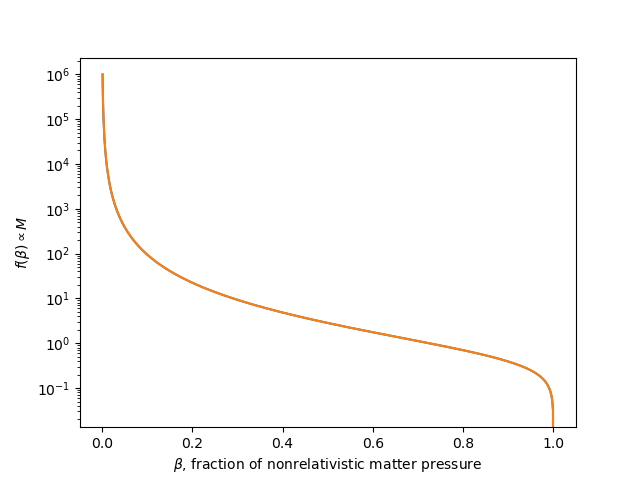
\includegraphics[width=\textwidth]{figures/beta_star_core_pressure.png}
\caption{A plot of \(f(\beta )\).}
\label{fig:beta-core-pressure}
\end{figure}
\todo[inline]{Figure made quickly, to improve by scaling it correctly, making it vector, setting the text in the right font.}

This makes sense intuitively: heavier stars reach higher temperatures and densities, so they have more radiation in the core. 

We know that for \(\beta \to 0\) the star is surely unstable, but the instability is actually reached earlier, since even before the gravitational binding energy being exactly zero large parts of the star can be flung out as stellar winds.
Proper considerations about what an appropriate critical value of \(\beta \) should be allow us to bound the stellar mass from above, at around \(50 M_{\odot}\). 

% [Plot of \(1 - \beta \) versus \(M / M_{\odot} \), showing this.]

\subsection{Degenerate electron gas}

Now, we will deal with the degenerate electron gas in stars, and see what is its effect on the minimum and maximum mass of a star.  

The distribution function of the electrons, which are fermions, is given by 
%
\begin{align}
  f(p) = \qty[\exp(\frac{\epsilon _p - \mu }{k_B T})+1]^{-1}
\,,
\end{align}
%
where \(\epsilon _p = \sqrt{m^2 c^{4} + p^2 c^2}\). With it, we can calculate the number density of electrons: 
%
\begin{align}
n_e = \frac{g_s}{h^3} \int \dd[3]{p} f(p)
\,,
\end{align}
%
where \(g_s\), the number of helicity states of the electron, is equal to 2.

We want to consider the degenerate case for this distribution, which corresponds to the saturation of all the low-energy configurations in phase space: this is known as a Fermi gas. 
As the temperature approaches zero, the phase space distribution approaches the configuration 
%
\begin{align}
f(p) = \lim_{T \to 0} \qty[\exp(\frac{\epsilon_p - \mu }{k_B T})+1]^{-1}= 
\begin{cases}
  1 \qquad \epsilon _p < \mu  \\
  0 \qquad \epsilon _p > \mu 
\,.
\end{cases}
\end{align}

The chemical potential yields a critical energy, known as the Fermi energy, \(\epsilon _F\), which is also tied to a Fermi momentum:
%
% Then, as \(T \rightarrow 0\) we get: \(f(\epsilon _p) = 1\) if \(\epsilon _p \leq \epsilon _F\) and \(f(\epsilon _p) = 0 \) if \(\epsilon _p > \epsilon _F\); we can express this energy in terms of the momentum: 
%
\begin{align}
  \epsilon_F^2 = c^2p_F^2 + m^2 c^{4}
\,.
\end{align}

The number density of electrons in this configuration is given by the integral mentioned before: since the distribution is spherically symmetric we have
%
\begin{align}
  n_e = 2 \int_{0}^{p_F} \dd{p} p^2 4 \pi \frac{1}{h^3}
  = \frac{8 \pi }{3} \qty(\frac{p_F}{h})^{3}
\,,
\end{align}
%
% where we have a factor of \(2\) to account for the spin-\(1/2\) nature of the electrons. 
% This means that 
which allows us to express the Fermi momentum in terms of the number density of electrons:
%
\begin{align}
  p_F = \qty(\frac{3n_e}{8 \pi })^{1/3} h
\,.
\end{align}

In natural units, this is roughly \(p_F \approx \num{6.6} \sqrt[3]{n_e}\).

The energy density is given by the expression
%
\begin{align}
  \rho = \frac{2}{h^3} \int_{0}^{p_F} 4 \pi p^2\dd{p} \epsilon _p
\,,
\end{align}
%
which we can consider in either the nonrelativistic or the ultrarelativistic limit --- the analytic integral is complicated and not very enlightening. 

\paragraph{Nonrelativistic limit}

% In the nonrelativistic limit we find 
In this limit the energy is approximately
%
\begin{align}
  \epsilon _p = mc^2 + \frac{p^2}{2m}
\,,
\end{align}
%
so in the computation we need to integrate a polynomial: the result is
%
\begin{align}
  \rho = n \qty(mc^2 + \frac{3}{10} \frac{p_F^2}{m})
\,,
\end{align}
%
where the first term corresponds to the rest-energy of the electrons, while the second gives their kinetic energy.
We have derived earlier the following expression for the pressure of a nonrelativistic gas:
%
\begin{align}
  P  = \frac{2}{3} \frac{E_k}{V}
\,,
\end{align}
%
% where \(E/V\) is the kinetic energy density. 
and \(E_k / V\) is precisely the kinetic energy density, the second term of the expression for the total energy density \(\rho \); 
so for our nonrelativistic Fermi gas we will have:
%
\begin{align}
  P = n \frac{p_F^2}{5m} 
\,.
\end{align}

Since the Fermi momentum \(p_F\) can be written as a function of the number density \(n_e\), so can the pressure \(P\): we find 
%
\begin{align}
P = \underbrace{\frac{h^2}{5m} \qty(\frac{3}{8 \pi })^{2/3}}_{K_{NR}} n_e^{5/3}
\,.
\end{align}

\paragraph{Ultra relativistic limit}

% In
% %
% \begin{align}
%   P = k_{NR} n^{5/3}
% \,,
% \end{align}
% %
% where 
% %
% \begin{align}
%   k_{NR} = \frac{h^2}{5m} \qty(\frac{3}{8 \pi })^{2/3}
% \,.
% \end{align}
%

In the relativistic case, on the other hand, we can approximate the energy as \(\epsilon _p \approx cp\), so the energy density will be given by 
%
\begin{align}
\rho = \frac{3}{4} n \rho _F c
\,.
\end{align}

In this case, we also know that the pressure becomes 
%
\begin{align}
  P = \frac{1}{3} \frac{E_k}{V}
\,,
\end{align}
%
so we find 
%
\begin{align}
P = \underbrace{\frac{hc}{4} \qty(\frac{3}{8 \pi })^{1/3}}_{K_{UR}} n^{4/3} 
\,.
\end{align}

\paragraph{Fermion gas classification}

We have discussed some expressions describing a non-relativistic or ultrarelativistic degenerate fermion gas. 

We have derived our results with the assumption \(T \to 0\), but a gas can behave very similarly with nonzero temperatures as well. 
What is the temperature threshold under which the gas behaves in a degenerate-like way?
We will not discuss how the transition region looks, but if \(k_B T \ll \epsilon _F\) then the gas behaves like a degenerate one, while if \(k_B T \gg \epsilon _F\) then there will be many unfilled gaps in the phase space distribution, so the gas will not be degenerate. 

Recall that \(p_F \propto n_e^{1/3}\): therefore, in a log-log plot of temperature \(T\) versus density of possible electron densities \(n_e\) we can draw a line distinguishing the degenerate and nondegenerate cases, with the critical temperature becoming higher for higher \(n_e\).

\todo[inline]{Is it really a straight line though? If the criterion is indeed to compare \(k_B T\) and \(\epsilon _p\) then I'd expect a curve, since \(\epsilon _F\) is not a polynomial function of \(p_F\)\dots}

% We make a plot: on the \(x\) axis we have the number density in \(\SI{}{m^{-3}}\), on the \(y\) axis we have the temperature in \(\SI{}{K}\).
Having distinguished the degenerate and nondegenerate regions, we can distinguish the relativistic and nonrelativistic ones: for the nondegenerate case, as is usual, we reach the relativistic condition if we increase the temperature. 

In the degenerate case this is not really the case: as long as the gas is degenerate, the temperature does not really matter, and the gas becomes relativistic when the Fermi energy \(\epsilon _F\) becomes larger than the mass of the fermion.
Since \(\epsilon _F\) is only a function of the number density, this means that the gas can become relativistic at arbitrarily low temperatures as long as it is dense enough.

\todo[inline]{Add plot --- maybe we can do a chromatic region plot, integrating numerically the distribution and coloring the region based on the fraction of relativistic particles, and for the degeneracy measure in some way how ``sharp'' the boundary is between the filled and unfilled regions?}

% We divide the plot into: 
% \begin{enumerate}
%     \item Classical UR: \(P \propto n k_B T\);
%     \item classical NR (like the Sun);
%     \item degenerate NR: \(P = K_{NR} n^{4/3}\)
%     \item degenerate UR. 
% \end{enumerate}

% Classical vs degenerate is marked by a line similar to \(T \sim n\), while we have NR for both \(T\) and \(n\) lower than certain critical values (since a degenerate gas can become ultrarelativistic even at low temperatures! this is the point).

\paragraph{Application to the Sun}

As we have discussed earlier, the core temperature, pressure and density of the Sun are related by the following relation:
%
\begin{align}
  P_c = \frac{\rho _c}{\overline{m}} k_B T_c
\,.
\end{align}

% and it can be (easily?) shown that 
The average mass which appears here is a function of the chemical composition of the interior: we can neglect all the metals and only consider the mass fractions of hydrogen (\(x_1 \)) and of helium (\(x_4 \)): 
%
\begin{align}
  \overline{m} = 2 m_H \times \frac{1}{1 + 3x_1 + 0.5 x_4}
\,.
\end{align}
%
% where \(x_{1, 4}\) are the concentrations of hydrogen and helium respectively. 

\todo[inline]{This expression works well in the limits of \(x_1 =1\) and \(x_4 = 1\), but where does it come from? I would have expected \(\overline{m} = (x_1 m_H  + x_4 m_{He} ) /2\)\dots}

The Clayton model gave us an expression for the central pressure \(P_c\), which we turned into one for the central temperature \(T_c\): 
%
\begin{align}
P_c &=\approx \qty(\frac{\pi }{36})^{1/3} G M^{2/3} \rho _c^{4/3} \\
 k_B T_c &\approx \qty(\frac{\pi }{36})^{1/3} G \overline{m}
  M^{2/3} \rho _c^{1/3}
\,,
\end{align}
%
however when deriving it we not consider the effect of the fact that the gas there may be at least party degenerate.

Let us consider a different approximation: suppose that the electrons in the core are fully degenerate and nonrelativistic, while the ions (whose density is \(n_i\), which by local neutrality is also equal to \(n_e = \rho _c / \overline{m}\)) are completely classical.\footnote{In order to see why it makes sense to consider them as classical while the electrons are degenerate, let us look at the fact that in the nonrelativistic approximation the Fermi energy is given by \(\epsilon _F = p_F^2 / 2m \sim m^{-1} n^{2/3}\), so the critical temperature needed for a Fermi gas to become degenerate depends on the number density as well as the mass of the particle: for a higher-mass particle, the Fermi energy is lower.

The electrons being degenerate means that the temperature of the core is (roughly speaking) lower than their Fermi energy; the Fermi energy of the ions however is at least three orders of magnitude lower, so it makes sense that it is not as low as the Fermi temperature of the ions.

In order to have some numbers at hand, with a number density like that of the core of the Sun the Fermi temperature for electrons is \(\sim \SI{11}{MK}\), while the Fermi temperature for protons is a measly \(\sim \SI{6000}{K}\). The actual temperature of the core is \(T_c \sim \SI{15}{MK}\), slightly above the Fermi temperature of electrons. It is close enough that modelling them as degenerate works, while the assumption of the ions being nondegenerate is completely valid.}
Our estimate for the central pressure will need to account for both electrons and ions:
% To estimate the maximum achievable central temperature we do: 
%
\begin{align}
  P_c = k_{NR} n_{e}^{5/3} + n_i k_B T_c
\,.
\end{align}
%

Let us equate this expression with the one given by the Clayton model for the central pressure: we find
%
\begin{align}
  \qty(\frac{\pi}{36})^{1/3} G M^{2/3} \rho_{c}^{4/3}
  &= k_{NR} \qty(\frac{\rho_c}{m_{H}})^{5/3} + \frac{\rho_{c}}{m_H} k_B T_c \\
  k_B T_c &= \underbrace{\qty(\frac{\pi}{36})^{1/3} G m_{H} M^{2/3}}_{A} \rho_{c}^{1/3} - \underbrace{k_{NR} m_H^{-2/3}}_{B} \rho _c^{2/3}
\,.
\end{align}
%

We can then ask what is the maximum temperature \(T_c\) we can reach for a given mass \(M\) if we vary the core density \(\rho _c\):
this can be calculated to be 
% (((np.pi/36) * ac.G**3 * ac.m_p**3 )/ (2 * ac.h**6 / 5**3 / ac.m_e**3 * (3/8 /np.pi)**2 /ac.m_p**2)).to(u.kg/u.m**3 / u.M_sun**2)
%
\begin{align}
\rho_{c}^{\text{max}} = (A/ 2B)^{3} \approx \SI{5e7}{kg/m^3} \qty( \frac{M}{M_{\odot}})^2
\,,
\end{align}
%
where we have 
%
\begin{align}
  k_B T_c = \frac{A^2}{4B} = \qty(\frac{\pi }{36})^{2/3} \frac{G^2m_H^{8/3}}{4 k_{NR}} M^{4/3}
  \approx \SI{5.7}{keV} \qty( \frac{M}{M_{\odot}})^{4/3}
\,.
\end{align}

% Now, we can set this temperature to be larger than the ignition temperature for any process we want, to see whether it will happen. 
This allows us to estimate the minimum mass a star needs to have in order to fuse hydrogen: we just need to set \(T_c\) to be equal to the ignition temperature \(T_c = T _{\text{ign}} \approx \SI{1}{keV}\) and we find
%
\begin{align}
  M _{\text{min}} = 
  \qty(\frac{36}{\pi })^{1/2} 
  \qty(\frac{4 k_{NR}}{G^2m_H^{8/3}})^{3/4}
  \qty(k_B T _{\text{ign}})^{3/4}
  \approx \SI{.27}{M_{\odot}}
\,.
\end{align}

This is a much better estimate than the one we found earlier since we are now accounting for the degenerate Fermi gas nature of the electrons in the core (this lowers the estimate, since it means that even at relatively low temperatures there will be electrons with high energy) and since we are computing the core density \(\rho _c\) instead of the average density \(\overline{\rho}\). 

\todo[inline]{The estimate is\dots still not great really, right? it is still 3 times larger than the correct value of \(\num{.08} M_{\odot}\)! How do we account for such a discrepancy?}

\paragraph{Expressing the result with coupling constants}

The gravitational potential energy between two hydrogen nuclei separated by a distance equal to their (reduced!) Compton wavelength \(r = \hbar / m_H c\) is 
%
\begin{align}
E_g = - \frac{G m_H^2}{r} = - \frac{G m_H^{3}c }{\hbar}
\,.
\end{align}

Comparing this to the rest energy of an electron, \(E = m_H c^2\), is the way to calculate the \emph{gravitational coupling constant} \(\alpha _G\), a dimensionless parameter quantifying the ``strength'' of the gravitational interaction between hydrogen nuclei:
%
\begin{align}
  \alpha_{G} = \frac{E_g}{E} =  \frac{G m_H^2}{\hbar c} \sim \num{5.9e-39}
\,.
\end{align}

In natural units, \(\alpha _G = m_H^2 / m_P^2\).

By a similar line of reasoning we find the electromagnetic coupling constant:
%
\begin{align}
  \alpha_{EM} = \frac{e^2}{4 \pi \epsilon_{0} \hbar c} \approx \frac{1}{137}
\,,
\end{align}
%
which is \emph{enormously} greater. 

In terms of the gravitational coupling constant the minimum mass we found can be written as 
%
\begin{align}
  M _{\text{min}} \approx
  16 \qty(\frac{k_B T _{\text{ign}}}{m_e c^2})^{3/4}
  \alpha_{G}^{-3/2} m_H
\,.
\end{align}

If \(T _{\text{ign}} \sim \SI{1.5e6}{K}\), one tenth of the temperature of the Sun, we find 
\todo[inline]{Is \SI{0.1}{keV} really enough to reach ignition? This seems to contradict what was said earlier\dots}
%
\begin{align}
  M _{\text{min}} \sim \num{.03} \alpha_{G}^{-3/2} m_H
\,.
\end{align}

We can apply a similar line of reasoning to the formula we found for the maximum mass: taking equation \eqref{eq:maximum-mass-main-sequence}  with a critical fraction of nonrelativistic matter of \(\beta = \num{.5}\) and \(\overline{m} = \num{.61} m_H\) we get a result which, once again, scales with \(\alpha _G^{-3/2} m_H\):
%
\begin{align}
  M _{\text{max}} \approx 56 \alpha_{G}^{-3/2} m_H
\,.
\end{align}

This hints to the fact that \(m_{*} = \alpha_{G}^{-3/2} m_H \) is an important characteristic mass for all of stellar evolution.

This is around \(\num{1.85} M_{\odot}\), and it corresponds to a number of nucleons of
%
\begin{align}
  N_{*} = \frac{m_{*}}{m_H} \approx \num{2e57}
\,.
\end{align}

\subsection{Full degeneracy and white dwarfs}

% Let us now suppose that the core of a star is held together by the pressure of degenerate electrons alone: we will discuss \emph{white dwarfs}.
White dwarfs are the remnants of low-mass stars who have exhausted the elements they are able to fuse in their core. They glow, emitting thermal radiation, which causes their temperature to slowly decrease until they become brown dwarfs. 

They are of interest to us since they allow us to apply the theory of degenerate Fermi gasses once more: they are very dense objects, since there is no fusion-induced pressure gradient inside them to balance gravity, and the electrons inside them form a degenerate gas.

% We define 
The number density of electrons inside a white dwarf is given by
%
\begin{align}
  n_e = Y_{e} \frac{\rho_{c}}{m_H}
\,,
\end{align}
%
where \(Y_e = (1 + x_1) /2\) quantifies the number of electrons per baryon (\(x_1 \) is the hydrogen mass fraction).

\todo[inline]{Why would \(Y_e\) be given by that expression? hydrogen has one electron per each baryon, but helium also has half an electron per baryon\dots If the white dwarf was exclusively hydrogen, would we not expect \(Y_e = 1/2\)?}

Let us start by assuming that the matter is nonrelativistic: then  
the pressure is given by
%
\begin{align}
  P = k_{NR} n_e^{5/3} = k_{NR} \qty(\frac{Y_e \rho_{c}}{m_H})^{5/3}
\,,
\end{align}
%
which as usual we compare to the results of the Clayton model:
%
\begin{align}
  P_c = \qty(\frac{\pi }{36})^{1/3} G M^{2/3} \rho_{c}^{4/3}
\,.
\end{align}

Equating these two we find
%
\begin{align}
  \rho_{c} \approx \frac{\num{3.1}}{Y_e^{5}} \qty(\frac{M}{m_{*}})^2 \frac{m_H}{(h / m_e c^2)^{3}}
\,.
\end{align}

% \todo[inline]{
%   Missing square on the \(M / m_*\)?
% }

If, on the other hand, we were to assume that the matter is ultrarelativistic the pressure would be given by
%
\begin{align}
P = k_{UR} n_e^{4/3} 
= k_{UR}\qty(\frac{Y_e \rho_{c}}{m_H})^{4/3}
\,,
\end{align}
%
so, instead of getting an expression for the central density \(\rho _c\), we would find
%
\begin{align}
  k_{UR} \qty(\frac{Y_e \rho_{c}}{m_H})^{4/3} \approx 
  \qty(\frac{\pi }{36})^{1/3} G M^{2/3} \rho_{c}^{4/3}
\,:
\end{align}
%
in this limit the expression becomes independent of \(\rho_{c}\)!

This gives us a limit mass, since as we increase the mass of a white dwarf which is not relativistic we increase its density and thus its temperature, making it closer to being relativistic, and this is the mass we get for the fully relativistic configuration (which is unstable because of the usual binding energy considerations).

The limit is known as the Chandrasekhar mass, the largest mass at which a fully degenerate white dwarf can support itself:
%
\begin{align}
  M_{CH} = 
  \qty(\frac{36}{\pi } )^{1/2} \qty(\frac{Y_e}{m_H})^2
  \qty(\frac{k_{UR}}{G})^{3/2} \approx 2.3 Y_e^2 m_{*} \approx 4.3 Y_e^2 M_{\odot} \approx 1.4 M_{\odot}
\,.
\end{align}

% This is the maximum mass of a white dwarf to remain stable, held together by the degeneracy pressure of electrons. 
% Above this, it becomes a neutron star.

% \todo[inline]{Pacciani includes some more detailed considerations about the Chandrasekhar mass.}

\todo[inline]{Something peculiar about the Chandrasekhar mass is that its derivation does not address the actual mechanism of the collapse (which is electron capture by nuclei, I think). If I understand correctly, this is because as \(M \to M _{\text{Ch}}\) the core density diverges, so something or other is \emph{bound} to happen, be it electron capture, the formation of an event horizon\dots}

\end{document}